%% principal.tex
%!TeX encoding = UTF-8

% Define o grau acadêmico e a língua principal do documento.
% ATENÇÃO: a última língua declarada é a língua principal do
% documento.
\documentclass[
    mestrado,              % Selecionar grau acadêmico: mestrado ou doutorado.
%    cotutela,              % Remover comentário se houver cotutela.
%    enlgish,
%    french,
%    spanish,
    brazil
]{feectex}

% Pacotes adicionais (adicione ou remova conforme sua
% necessidade). Visite o site https://www.ctan.org para
% consultar outros pacotes. Pacotes marcados com ! são,
% em essência, desnecessários: livre-se deles!
\usepackage{amsmath, amsfonts, amssymb}
\usepackage{pdfpages}
\usepackage{hyperref}
\usepackage{lmodern}
\usepackage{subcaption}
\usepackage{duckuments}     % !
\usepackage{lipsum}         % !

% Diretório onde se encontram as imagens utilizadas no trabalho.
% O comando pode ser modificado para incluir diversos diretórios:
%   \graphicspath{{dir1/}{dir2/}...}
\graphicspath{{./figuras/}}

%
% Informações da obra.
%

% Qual é o título da obra?
\titulo{Título da Obra}

% Qual é o seu nome e o número do seu RA?
\autora{Nome da Autora}
%\autor{Nome do Autor}
\ra{999999}

% Qual é o título e o nome da sua orientadora ou orientador?
\orientadora{Profa. Dra. Nome da Orientadora}
%\orientador{Prof. Dr. Nome do Orientador}

% Qual é o título e o nome da sua coorientadora ou coorientador?
% Se não houver, comente ambas as linhas abaixo.
% \coorientadora{Profa. Dra. Nome da Coorientadora}
\coorientador{Prof. Dr. Nome do Coorientador}

% Qual é a universidade e o instituto ou faculdade?
\universidade{Universidade Estadual de Campinas}
\institutooufaculdade{Faculdade de Engenharia Elétrica e de Computação}

% Qual é o nome da universidade de cotutela? Se houver,
% modificar a opção na declaração da classe acima
% (\documentclass(...)). Caso contrário, comente a linha abaixo.
% \universidadecotutela{Nome da Universidade (País)}

% Qual é a cidade onde foi ou será realizada a defesa?
\local{Campinas}

% Qual data foi ou será realizada a defesa?
\diadefesa{XX}
\mesdefesa{janeiro}
\anodefesa{20XX}

% Qual é a área de concentração do trabalho? Selecione uma.
% Estas são as áreas de concentração informadas no Catálogo
% dos Cursos de Pós-Graduação Strictu Sensu - UNICAMP -
% 2023, no Programa de Engenharia Elétrica.
% \areaconcentracao{Automação}
% \areaconcentracao{Eletrônica, Microeletrônica e Optoeletrônica}
% \areaconcentracao{Engenharia Biomédica}
\areaconcentracao{Engenharia de Computação}
% \areaconcentracao{Energia Elétrica}
% \areaconcentracao{Telecomunicações e Telemática}

% Quais são os títulos e os nomes dos componentes da banca
% examinadora? (Por enquanto, é necessário repetir o título
% e o nome da orientadora ou orientador aqui.)
\bancaexaminadora{%
    Prof. Dr. Nome do Orientador (Presidente) \\%
    Prof. Dr. Nome do Primeiro Membro \\%
    Prof. Dr. Nome do Segundo Membro
    % Prof. Dr. Nome do Terceiro Membro \\%
    % Prof. Dr. Nome do Quarto Membro
}

\begin{document}
    % \hyphenation{}

    % Elementos pré-textuais:
    %   capa;
    %   folha de rosto;
    %   ficha catalográfica;
    %   folha de aprovação;
    %   dedicatoria;
    %   agradecimentos;
    %   epigrafe;
    %   resumo / abstract;
    %   lista de ilustrações;
    %   lista de tabelas;
    %   lista de abreviaturas e siglas;
    %   lista de simbolos;
    %   sumário.
    % Comente os elementos não utilizados no seu trabalho.
    \imprimircapa
    \imprimirfolhaderosto
    \imprimirfichacatalografica{ficha-catalografica.pdf}
    \imprimirfolhaaprovacao
    \imprimirdedicatoria
    \imprimiragradecimentos
    \imprimirepigrafe
    \imprimirresumo
    \imprimirlistailustracoes
    \imprimirlistatabelas
    \imprimirlistaabreviaturassiglassimbolos
    \imprimirsumario

    % Elementos textuais.
    \textual
    \part{Primeira Parte}
    %!TeX root = ../principal.tex
%!TeX encoding = utf-8
\chapter{Classe FEECTeX}
\label{cap1}

\section{Citações}

Considerando que as referências estejam armazenadas no arquivo \textit{bibliografia.bib} na pasta raíz, as citações podem ser feitas através dos comandos:

\begin{itemize}
    \item \verb|\citar{<chave#1>, <chave#2>, ..., <chave#n>}|;
    \item \verb|\citarautora{<chave>}| ou \verb|\citarautor{<chave>}|;
    \item \verb|\citarano{<chave>}|.
\end{itemize}

Exemplos:

\begin{itemize}
    \item \verb|\citar{autor, autora}| produz \citar{autor, autora};
    \item \verb|\citar| \verb|autora{autora}| produz \citarautora{autora};
    \item \verb|\citarano{autora}| produz \citarano{autora}.
\end{itemize}

Citação direta com mais de 3 linhas, por sua vez, é feita através do ambiente \verb|citacao|, ou seja, \verb|\begin{citacao}|\dots\verb|\end{citacao}|.

\begin{citacao}
    Nam dui ligula, fringilla a, euismod sodales, sollicitudin vel, wisi. Morbi auctor lorem non justo. Nam lacus libero, pretium at, lobortis vitae, ultricies et, tellus. Donec aliquet, tortor sed accumsan bibendum, erat ligula aliquet magna, vitae ornare odio metus a mi. Morbi ac orci et nisl hendrerit mollis. Suspendisse ut massa. Cras nec ante. Pellentesque a nulla. Cum sociis natoque penatibus et magnis dis parturient montes, nascetur ridiculus mus. Aliquam tincidunt urna. Nulla ullamcorper vestibulum turpis. Pellentesque cursus luctus mauris.
\end{citacao}

\section{Notas de Rodapé}

As notas de rodapé são declaradas através do comando \verb|\footnote{<nota>}|, por exemplo: a classe \feectex é derivada da classe abntex2\footnote{O abnTeX2 é uma evolução do abnTeX -- ABsurd Norms for TeX.}.

\section{Abreviaturas e siglas}

A lista de abreviaturas e siglas é gerada automaticamente. Para que isso aconteça, basta que os comandos \verb|\abreviatura{<abreviatura>}|\verb|{<definição>}|, \verb|\sigla| \verb|{<sigla>}{<definição>}| sejam encontrados durante a preparação do documento PDF.

Exemplos:

\begin{itemize}
    \item \verb|\sigla{ABNT}{Associação Brasileira de Normas Técnicas}|
    \item \verb|\abreviatura{Dr.}{Doutor}|
\end{itemize}

\sigla{ABNT}{Associação Brasileira de Normas Técnicas}
\abreviatura{Dr.}{Doutor}

\section{Símbolos}

Assim como lista de abreviaturas e siglas, a lista de símbolos também é gerada automaticamente. Da mesma maneira, basta que o comando \verb|\simbolo<símbolo>}| \verb|{<definição>}| seja encontrado ao longo da preparação do documento PDF para que isso aconteça.

Exemplo:

\begin{itemize}
    \item \verb|\simbolo{$\mathbb{R}$}{Conjunto dos números reais}|
\end{itemize}

\simbolo{$\mathbb{R}$}{Conjunto dos números reais}

\section{Tabelas}

\begin{table}[h]
    \centering
    \begin{tabular}{c | c}
        \hline
        Autor & Obra \\
        \hline
        Akira Toriyama & Dragon Ball \\
        Carlos Drummond de Andrade & De Notícias \& Não Notícias Faz-Se a Crônica
    \end{tabular}
    \caption[Tabela]{Tabela de autores e obras.}
    \label{table:1}
\end{table}

\section{Figuras}

O tamanho das imagens pode ser escolhido através dos comandos \verb|width| e \verb|scale|.

\begin{figure}
    \centering
    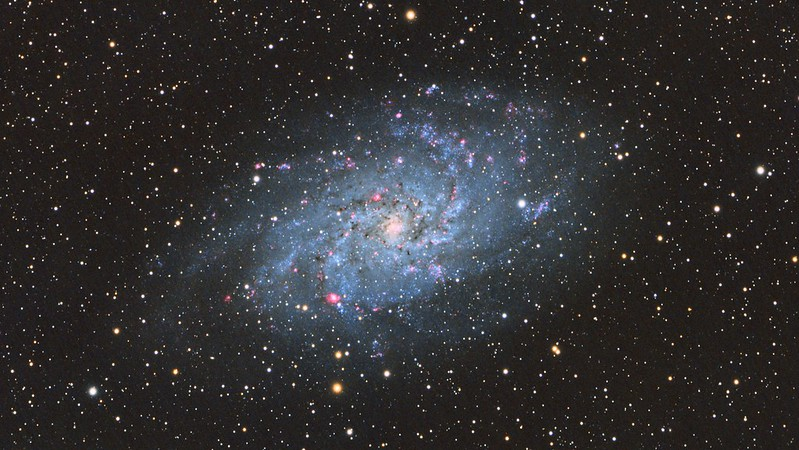
\includegraphics[width=0.8\textwidth]{capitulo-1/28421613139_a4472645e5_c.jpg}
    \caption[Galáxia M33]{Galáxia do Triângulo M33.}
\end{figure}

\subsection{Múltiplas figuras}

\begin{figure}[t]
    \centering
    \begin{subfigure}[b]{0.3\textwidth}
        \centering
        \includegraphics[width=\textwidth]{example-image-duck}
        \caption{Primeiro pato.}
    \end{subfigure}
    \hfill
    \begin{subfigure}[b]{0.3\textwidth}
        \centering
        \includegraphics[width=\textwidth]{example-image-duck}
        \caption{Segundo pato.}
    \end{subfigure}
    \hfill
    \begin{subfigure}[b]{0.3\textwidth}
        \centering
        \includegraphics[width=\textwidth]{example-image-duck}
        \caption{Terceiro pato.}
    \end{subfigure}
       \caption{Três patos juntos.}
\end{figure}


    % Elementos pós-textuais:
    %   bibliografia / referências;
    %   apêndices;
    %   asnexos.
    % Comente os elementos não utilizados no seu trabalho.
    \postextual
    \bibliography{bibliografia}
    \apendices
    %!TeX root = ../principal.tex
%!TeX encoding = utf-8
\chapter{Lorem Ipsum}
\label{apendice}

Texto do apêndice.

    \anexos
    %!TeX root = ../principal.tex
%!TeX encoding = utf-8
\chapter{Aliquam Dignissim}

Texto do anexo.

\end{document}
